\subsection{Experiment Setup}
\label{sec:experiments}

In this subsection, we describe the testbed for monitoring video streaming traffic under various network conditions.
%Next, we describe the process for collecting video traffic data.

\subsubsection{Testbed}
Similar to the previous chapter, we have designed our testbed to observe streaming video traffic from YouTube. 
The monitoring is performed at the client end, where the video is played out in a browser.
Since we want to study the adaptation behavior when bandwidth changes, it is important that we can control the bandwidth available.
We do not have control over the available bandwidth to the YouTube server over the Internet, but we could place a bandwidth throttler that can restrict the bandwidth available to the client below what is actually available.
The complete testbed architecture is shown in \fig\ref{fig:experimentalSetup}.

\begin{figure}[!t]
	\centering
	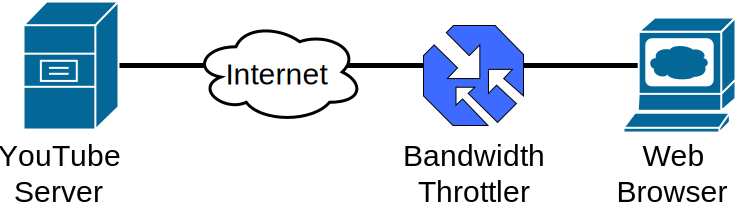
\includegraphics[width=0.7\linewidth]{img/experimentalSetup}
	\caption{Experimental testbed}
	\label{fig:experimentalSetup}
\end{figure}

The bandwidth throttler component is implemented using the {\tt NetFilterQueue} Linux library.
The {\tt iptables} tool, which uses {\tt NetFilterQueue}, is used to manipulate the network bandwidth available for the web browser.
%To simulate a given bandwidth, we delay the network packets before it reaches the application (browser).
Since we are comparing the performance of \ac{QUIC} and \ac{TCP}+\ac{TLS}, we need to play the videos at a browser which has support for both \ac{QUIC} and \ac{TCP}+\ac{TLS}. Google's Chrome browser supports both the protocol stacks that can be configured using {\tt chrome://flags}. We also use the command line tool \texttt{speedtest-cli} to periodically monitor the available network bandwidth at the backbone. If the backbone bandwidth drops more than $10$ Kbps from the current throttler bandwidth, we discard that data and initiate streaming of the corresponding video from the scratch.
%. Under this scenario, the streaming procedure for that video has been initiated again from the scratch.  

\subsubsection{Data Collection Process}
We use the {\tt NetMonitor} tool available as part of the browser developer tools to collect the traffic related information.
We focus on the \ac{HTTP} request-response messages, which are stored as \ac{HAR} file that contain information in \ac{JSON} format. In our data collection process, we start the bandwidth throttler before accessing a video for playback in a browser. We play the video till the end, while collecting the \ac{HAR} file containing the relevant traffic information.
The throttler is designed to switch bandwidth levels from $64$ Kbps to $1424$ Kbps in steps of $340$ Kbps at every $220$ seconds. Once the bandwidth reaches to $1424$ Kbps, the throttler starts decrementing the bandwidth at the same rate. 
%This is indeed a circular procedure that keeps on running at the background during the streaming of every video file. 
%The entire process is automated through a script. 
We use Google Chrome Remote Interface\footnote{\url{https://github.com/cyrus-and/chrome-remote-interface} (\lastaccessedtoday)} plugin to automatically open the browser and load a video.
To capture the \ac{HAR} files, we use \texttt{chrome-har-capturer}\footnote{\url{https://github.com/cyrus-and/chrome-har-capturer} (\lastaccessedtoday)} plugin.
Since \texttt{chrome-har-capturer} is not event driven, and must be configured to store a data for a fixed time window, we specify the video length with few additional minutes as the time to capture data. The length of the video can be found using YouTube video info \ac{API}\footnote{\url{https://www.youtube.com/get_video_info} (\lastaccessedtoday)}.
The additional wait also accounts for any rebuffering events when the video would stall.
%All these features allow in automatically playing large number of videos and capturing the data.

 
\begin{comment}
We want to test how YouTube performs with various network condition from the edge of the Internet. To do this, we set up our testbed as shown in \fig\ref{fig:experimentalSetup}. There are four components in our testbed. They are YouTube server, the Internet, bandwidth throttler and a QUIC supported browser. Although we do not have any control over the YouTube server, it is an essential part of the testbed as we are performing experiments on YouTube only.

To perform various experiment efficiently, we need a high-quality Internet connection. We do not want an Internet connection to be a bottleneck. It should support the speed we needed to perform the experiments. To ensure high-speed and high-quality Internet connection, we perform our experiments on the Institute's Internet backbone. Then again, we monitor the connection quality throughout the experiments.

As we want to perform experiments for various network conditions, we need to emulate those network conditions. To simulate the realistic bandwidth limited setting, we throttle the available link bandwidth. Linux system have a traffic shaper name {\fontfamily{qcr}\selectfont tc}. But there are some issue with {\fontfamily{qcr}\selectfont tc} for ongoing connections. So, we have designed our bandwidth throttler. There is a open Linux library, {\fontfamily{qcr}\selectfont NetFilterQueue}, available to perform various task on network packet from user space with the help of {\fontfamily{qcr}\selectfont iptables}. We took help of this tools to throttle bandwidth. In this tool, we hold packets in a queue and release them according to the required bandwidth.

\begin{figure}[h!]
\centering
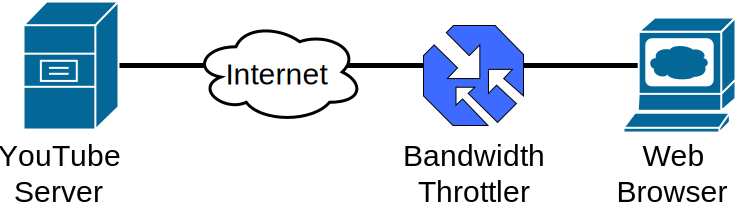
\includegraphics[width=\linewidth]{img/experimentalSetup}
\caption{Experimental testbed}
\label{fig:experimentalSetup}
\end{figure}

As we are experimenting YouTube performance for the web, we need a browser. We want to compare YouTube's performance when it is using QUIC as underlying protocol with when it is using TCP+TLS as the underlying protocol. All the browsers support TCP+TLS, but there are only two browsers available which support QUIC as the underlying protocol. These are Chromium browser and Google Chrome browser. Both the browsers developed by Google only and they are almost identical in every aspect. However, Google Chrome is more popular than Chromium browser. So, we choose Google Chrome to perform the experiments. Both the browser have the option for enabling or disabling QUIC using {\fontfamily{qcr}\selectfont chrome://flags}. We perform experiments using both enabling the flag and disabling it for QUIC and TCP+TLS respectively.

Above mentioned details is the primary requirement for the experiments to be performed. However, we need to automate the process and collect relevant data out of these experiments. In following subsections, we discuss the data collection procedure and the automation procedure.


\subsection{Data Collection Procedure}
Almost all the popular browsers have developer tools. In this tool set, a user can perform various experiments on their website to observe a website performance. Among these tool set, one tool call {\fontfamily{qcr}\selectfont NetMonitor} (name of this tool is browser dependent). In this tool, one can see various information regarding HTTP request and response. These pieces of information are request and response headers and body, different time (like DNS lookup, connection establishment, waiting time before response arrives and time requires to receive the response). Most of the network tool have support for storing these pieces of information on the disk. It store those information in a format call HAR (\textbf{H}TTP \textbf{Ar}chive). HAR is JSON format, so it is easy to read by any text editor or programming language. In our experiments, we stored the HARs of each video and analyzed later.

For each experiment, we first run throttler program, then open a browser and loads the desired YouTube video. Then we waited till the video playback finishes. After completion of a video playback, we stored the HAR and closed the browser and throttler program. Throttler program not only throttle the bandwidth, but it also changes the bandwidth level. The bandwidth levels used are from 64 Kbps to 1424 Kbps, in a step of 340Kbps. Each level of bandwidth is kept fixed for 220 seconds. This whole procedure can be done manually. However, to collect data for a large number of videos, manual work can be very cumbersome and a waste of time. So, we automate the entire procedure.

\subsection{Automation procedure}
Automation is the one of the essential requirement to perform experiments. So, we have developed a python script which does all the step mentioned in the last subsection. For us, the major challenge in automation was automation of Google Chrome browser. To start Google Chrome browser and load the required video we use Google Chrome Remote Interface\footnote{\url{https://github.com/cyrus-and/chrome-remote-interface} (\lastaccessedtoday)} plugin. However, this plugin does not have access to the network monitor. So, to store HAR from network monitor of Google Chrome browser, we use chrome-har-capturer\footnote{\url{https://github.com/cyrus-and/chrome-har-capturer} (\lastaccessedtoday)} plugin. However, chrome-har-capture have a limitation. One can not trigger when to store HAR to disk. One has to give a waiting time at the very beginning, and this plugin will wait for that long before saving the HAR in the disk. So, we first find out the duration of the video using YouTube vide info api\footnote{\url{http://www.youtube.com/get_video_info} (\lastaccessedtoday)} then put waiting time as video length + 5 minutes. We have waited 5 minutes extra so the video can finish its playback even if playback stalls for rebuffering in between. We also turned off autoplay next feature of YouTube, so that it does not start playing some other video after completion of the desired video.

After automating all this, it becomes easier to run experiments for multiple videos unattended. In the following section, we discuss the different statistics of the videos and analysis parameters.


%As only Google Chrome browser and Chromium browser support QUIC, we need to perform experiments using one of them. Considering available plugins and APIs, there doesn't have any difference between Google Chrome browser and Chromium browser. So we choose Google Chrome browser to perform our experiment as it is more widely used over Chromium browser. To collect HAR from Google Chrome programmatically we use chrome-har-capturer\footnote{\url{https://github.com/cyrus-and/chrome-har-capturer} (\lastaccessedtoday)} and to automate this experiments we use Google Chrome Remote Interface\footnote{\url{https://github.com/cyrus-and/chrome-remote-interface} (\lastaccessedtoday)}.
%
%In order to simulate the  realistic bandwidth limited setting we throttle the available link bandwidth. Although Chrome support throttling in network monitor, there is no suitable way to change it from script. Therefore we make use of the throttler developed  with the Unix library {\fontfamily{qcr}\selectfont NetFilterQueue} \cite{citation-2-name-here}. It is a user-space library that provides an API to handle packets, which have been queued by the kernel packet filter, as per user requirement. Based on this library, traffic shaper was developed to control link bandwidth. However, we need to continuously monitor and ensure that the backbone network has sufficient bandwidth so that the overall link bandwidth is controlled only by the throttling procedure. We load a YouTube video, wait for the video to finish and then save the HAR and other information to the disk. During video playback, we also control network bandwidth by progressively increasing the bandwidth followed by a sudden decrease and the cycle repeats. The bandwidth levels used are from 64 Kbps to 1424 Kbps, in a step of 340Kbps. Each level of bandwidth is kept fixed for 220 seconds.
%
%\begin{figure}[h]
%	\centering
%	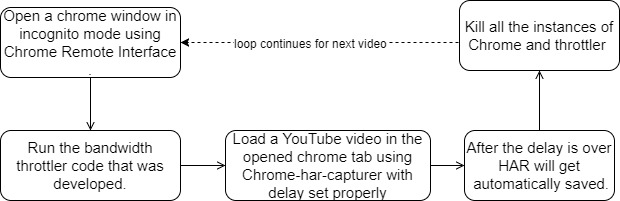
\includegraphics[width=\linewidth]{img/setup}
%	\caption{Experimental Set-up}
%	\label{fig:mesh11}
%\end{figure}
%
%\section{Dataset}
\end{comment}
\begin{comment}
\subsection{Extract Useful Information from the HTTP Headers}

From the HAR traces, we observe that YouTube uses a video playback request to grab the media data from the server. URLs for these video playback requests contain 35 parameters and their values:  \textit{pl, dur, expire, sver, gir, pcm2cms, mime, itag, signature, ipbits, source, keepalive, mt, mv, ms, mm, mn, key, clen, requiressl, lmt, initcwndbps, id, upn, sparams, fexp, ip, cpn, alr, ratebypass, c, cver, range, rn, and rbuf.} By close inspection of these parameters, we observe that the HTTP requests and responses are forwarded separately for the audio channel and the video channel. The value of the parameter \textit{mime} indicates whether the request is for audio channel or for video channel. Then, we figure out that the parameter \textit{itag} actually indicates the video quality for which a DASH request is made. YouTube samples every video under different video quality levels based on its resolution, bit rate and encoding techniques used for sampling, and assigns a numeric level to every quality, which is the itag value. The mapping between a particular \textit{itag} value and the corresponding video resolution, bit-rate and encoding parameters are given in \tbl\ref{table:2}.

\begin{table}[ht!]
	\centering
	\begin{tabular}{||c |c |c||} 
		\hline
		\textbf{Itag} & \textbf{Resolution} & \textbf{Type}  \\ [0.5ex] 
		\hline\hline
		160 & 256x144 & video/mp4 \\ 
		\hline
		278 & 256x144 & video/webm \\ 
		\hline
		133 & 426x240 & video/mp4 \\ 
		\hline
		242 & 426x240 & video/webm \\ 
		\hline
		134 & 640x360 & video/mp4 \\ 
		\hline
		243 & 640x360 & video/webm \\ 
		\hline
		135 & 854x428 & video/mp4 \\ 
		\hline
		244 & 854x428 & video/webm \\ 
		\hline
	\end{tabular}
	\caption{Information about itags}
	\label{table:2}
\end{table}

The behavior of these parameters under different scenarios like {\em Multiple videos multiple sessions, Single video multiple sessions, Single video single session} was observed. When a value does not change over multiple videos multiple sessions, then it indicates that the parameter does not take part in video adaptation procedure, and it basically forwards some static information, like the device and the operating system related information. If the value of a parameter changes for multiple video multiple sessions, but does not change for single video multiple sessions, then we can say that it is a video specific parameter.  If the value of a parameter changes for single video multiple sessions, but does not change for a single video single session even if the network quality changes, then we can say that it is session specific. The parameters that change only in this scenario when we change the link bandwidth, indicate that they possibly take part in the video adaptation process. From here, it was figured out in that  \textit{clen, dur, itag, lmt, mime, rbuf, rn, signature and range} are such parameters. However through close inspection, we find the parameters  \textit{mime} and  \textit{signature} relate to video channels, as we already discussed. Further the parameter  \textit{dur} denotes video duration, and it was observed that it changes only at microsecond order which is due to the change in video encoding technique. Consequently, we go for comparison of the other parameters between QUIC and TCP - \textit{ clen, itag, lmt, range, rbuf and rn.} It was observed that for the single video single session scenario, \textit{rbuf, rn} and \textit{range} change even for a single \textit{itag}. On the other hand, parameters like \textit{clen} change overall, but remain constant for a single \textit{itag} value.

\end{comment}
